\section{Analysis}

\begin{figure}
    \centering
    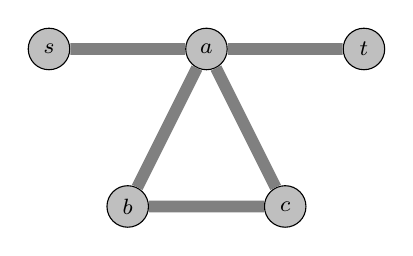
\begin{tikzpicture}
        \tikzstyle{every node}=[circle, fill=lightgray, draw=black, inner sep=2pt, minimum size=1.5em, font=\footnotesize, text=black]
        \tikzstyle{edge}=[gray, line width=1.5mm]
    
        \node (s) at (0,2) {$s$};
        \node (a) at (2,2) {$a$};
        \node (b) at (1,0) {$b$};
        \node (c) at (3,0) {$c$};
        \node (t) at (4,2) {$t$};
    
        \draw[edge] (s) -- (a) -- (b) -- (c) -- (a) -- (t);
    \end{tikzpicture}
    \caption{No odd $s$-$t$-path exist, yet we still have many odd $s$-$t$-walks.}
    \label{figure:small2}
 \end{figure}

Consider \Cref{figure:small2}. There are no odd paths from $s$ to $t$, but we have an infinite amount of odd walks by utilizing the cycles $[a,b,c]$ or $[a,c,b]$ an odd number of times to offset the parity. Our algorithm would perhaps first find an odd walk to $a$, then an even walk to $b$, then an odd walk to $c$, then an even walk to $a$, and lastly an odd walk to $t$. This is one of the two odd $s$-$t$-walks of minimum cost. However, $a$ is visited twice in the walk, once for each parity, and the resulting walk is not a path. Therefore, this algorithm cannot be used to solve \textsc{Shortest Odd Path}.

The main limitation of the algorithm is that the edges in the input graph must have either non-negative weights or no weights at all. Otherwise, we cannot guarantee that \pyth{even_dist[u]} and \pyth{odd_dist[u]} have their final, correct values when we scan a vertex $u$. Note that unlike most other algorithms shown in this thesis, this algorithm does not require the input graph to be undirected, it may also be directed.

\begin{theorem}
    Let $(G,s,t)$ be an instance of \textsc{Shortest Odd Walk}, let $n := |V|$ and let $m := |E|$.\\
    Claim: the algorithm runs in time at most $O(m \cdot \log m)$, or $O(m \cdot \log n)$ if the graph is simple.
    \begin{proof}
        Because of our \pyth{odd_done} and \pyth{even_done} arrays, we can guarantee that each vertex is scanned at most twice, once for each parity. For each scan, we loop through each of the neighbors in linear time and consider putting them in the queue. The total cost of the scans is therefore at most $O(m)$. A vertex may be put into the queue many times before it is scanned, in the worst case once for each of its neighbors. That means that we put vertices in the queue at most $O(m)$ times, for a total cost of $O(m)$, and removing all of them takes a total of $O(m \cdot \log m)$. 
        
        The algorithm runs in time at most $O(m) + O(m \cdot \log m) = O(m \cdot \log m)$, which shows the first part of the claim.
        
        If the graph is simple we may simplify the complexity further: $O(m \cdot \log m) \subseteq (m \cdot \log n^2) = O(m \cdot 2 \cdot \log n) = O(m \cdot \log n)$, which shows the second part of the claim.
    \end{proof}
\end{theorem}

To test how well the algorithm scales, we generate 200 Delaunay graphs of sizes 1000, 2000, 3000, and so on until 200k. We explain how these graphs are generated in \Cref{section:benchmarking}. For each graph, we have estimated a source and target with the maximum shortest path between them, and run our \textsc{Shortest Odd Walk} algorithm. We take the median running time of 10 runs and plot the results below. We have also tried to find constants to convert the $O(m \cdot \log n)$ theoretical complexity into a comparable function and plotted it next to the real practical results.

\begin{center}
    \includesvg[width=0.9\textwidth]{figures/bench_plots/shortest odd walk.svg}    
\end{center}

As we can see, the algorithm easily solves \textsc{Shortest Odd Walk} on graphs of 200k+ vertices in less than 100ms. There is only a slight upward curve as the inputs grow, which is what we expect from a linearthmic theoretical running time.

We also benchmark the algorithm on seven graphs from real-life scenarios, as seen in the table below. Four of the synthetic Delaunay graphs are added for comparison. Each graph is run 20 times, and we take the average running times and show them in the table below. See \Cref{section:benchmarking} for more details on how the benchmarking is done.

\begin{center}
    \begin{tabular}{|l | r | r | r |} 
        \hline
        Graph & n & m & Time spent \\ [0.5ex] 
        \hline\hline
        Power BCSPWR09 \cite{graph:bcspwr09-ca-citeseer} & 1723 & 2394 & $<1\text{ms}$ \\
        \hline
        Oldenburg \cite{graph:oldenburg-sf-cal-san-roads-etc} & 6106 & 7035 & 1ms \\ 
        \hline
        San Joaquin County \cite{graph:oldenburg-sf-cal-san-roads-etc} & 18263 & 23874 & 3ms \\
        \hline
        Cali Road Network \cite{graph:oldenburg-sf-cal-san-roads-etc} & 21048 & 21693 & 3ms \\
        \hline
        Musae Github \cite{graph:musae-github} & 37700 & 289003 & 18ms \\
        \hline
        SF Road Network \cite{graph:oldenburg-sf-cal-san-roads-etc} & 174956 & 223001 & 46ms\\
        \hline
        Ca Citeseer \cite{graph:bcspwr09-ca-citeseer} & 227321 & 814137 & 132ms \\
        \hline
        \hline
        Delaunay 50k & 50000 & 149961 & 15ms \\
        \hline
        Delaunay 100k & 100000 & 299959 & 38ms \\
        \hline
        Delaunay 150k & 150000 & 449965 & 64ms \\
        \hline
        Delaunay 200k & 200000 & 599961 & 92ms \\
        \hline
    \end{tabular}
\end{center}

As we can see, the algorithm does very well on all the inputs, and notably has no trouble solving for the Ca Citeseer graph of 227k vertices and 814k edges in less than 150ms. These results are excellent. Despite having a similar complexity to the other algorithms in this thesis, this algorithm is still by far the fastest in practice.

Though we discovered it independently, the algorithm is not particularly groundbreaking or in any way creative. Therefore, we do not expect it to be original. It is, however, quite fast, and we are happy with that. The main reason we include it in this thesis is because of its pedagogical value in introducing our main topic: \textsc{Shortest Odd Path}. \todo{Her burde vi finne en eksisterende algoritme og referere til den.}
